\documentclass[a4paper]{article}
\usepackage[italian]{babel}
\font\TitleFont=cmr12 at 50pt
\font\AuthFont=cmr13 at 20pt
\font\ChapFont=cmr12 at 30 pt
\usepackage{titling}
\usepackage{graphicx}
\usepackage[section]{placeins}
\usepackage{tabularx}

\title {{\TitleFont Esercizio 2}}
\date{3 Luglio 2019}
\author{{\AuthFont Alessandro D'Amico}}


\renewcommand\maketitlehooka{\null\mbox{}\vfill}
\renewcommand\maketitlehookd{\vfill\null}

\begin{document}
\begin{titlingpage}
\maketitle
\end{titlingpage}
\tableofcontents
\newpage
\section{Introduzione al problema}
Lo scopo di questo esercizio e' verificare i vantaggi e gli svantaggi di due strutture dati: \textbf{Alberi binari di ricerca (ABR)} ed \textbf{Alberi rosso-neri (ARN)} e' quindi necessario studiare il tempo di esecuzione delle varie operazioni tipiche su strutture dati
\section{Caratteristiche teoriche di algoritmi e e strutture utilizzate}
Le due strutture dati sono ad albero e pertanto prevedono l'esitenza di un nodo detto "radice" (all'apice di essi). Ogni nodo ha un attributo \textbf{p} corrispondente al padre, un attributo \textbf{left} corrispondente al proprio figlio sinistro ed un attributo \textbf{right} corrispondente al figlio destro
\newline
\textbf{ABR}: Negli alberi binari di ricerca si ha che il figlio sinistro (left) e' minore del padre, mentre il figlio destro (right) e' maggiore del padre. L'altezza dell'albero non ha un upper bound e dunque, nel caso i valori siano stati inseriti in ordine (crescente o decrescente), l'albero risulta sbilanciato; essendo che la ricerca e l'inserimento scendono l'albero livello per livello, nel caso critico appena citato il tempo richiesto per tali operazioni puo' essere molto elevato.   
\newline
\textbf{ARN}: Derivano dagli ABR, ma a differenza di essi i nodi che lo compongono sono dotati dell'attributo "color", grazie a cui si puo mantenere bilanciato l'albero (e' dimostrabile che h$_{alberoRN}\leq2lg(n+1)$): per mantenere tale caratteristica ad ogni inserimento bisogna pero' chiamare la funzione \textbf{fix-up}, il che ha un costo a volte non trascurabile.

\section{Prestazioni attese}
Le prestazioni attese per gli algoritmi relativamente ad ABR ed a ARN sono riportate nella tabella sottostante. Non eseguiremo test di \textbf{Delete} poiche' avremmo conclusioni affini con \textbf{Search} ed \textbf{Insert}	
\newline
\newline
	\begin{tabularx}{10cm}{|X|X|X|X|}
	\hline
	Struttura dati & Search & Insert & Delete  \\
	\hline
	\textbf{ABR} & $O(h)$  & $O(h)$ & $O(h)$  \\
	\hline
	\textbf{ARN} &  $O(\log{}n)$ & $\Theta(\log{}n)$ & $O(\log{}n)$\\
	\hline
	\end{tabularx}
\section{Esperimenti}
Sono stati effettuati in totale 4 esperimenti (tutti prevedono l'utilizzo di dataset da 0 a 50000 numeri interi positivi), in ognuno dei quale vengono confrontati ABR ed ARN:
\newline
\newline
\textbf{1.} Inserimento di dataset di numeri random 
\newline
\textbf{2.} Inserimento di dataset di numeri ordinati in modo decrescente 
\newline
\textbf{3.} Ricerca su alberi generati da dataset di numeri random
\newline
\textbf{4.} Ricerca su alberi generati da dataset di numeri ordinati in modo decrescente
\newline


\section{Documentazione del codice}
\newpage
\section{Risultati}
Sono stati effettuati i test con piu set di numeri (set da 10, 100, 1000 valori), tenendo conto del fatto che la dimensione di ogni singolo numero (in termini di cifre) non incide sulla nostra analisi (trattandosi di algoritmi per confronto (non si tiene conto del max o del min). E' dunque necessario distinguere due casi, a seconda che si usi un set ridotto o un set di grandi dimensioni. 
\subsection{Inserimento - Caso medio (Input Random)}
Dalla Figura \ref{fig:InsMedio} 	

 		\begin{figure}[!htb]
		\centering
		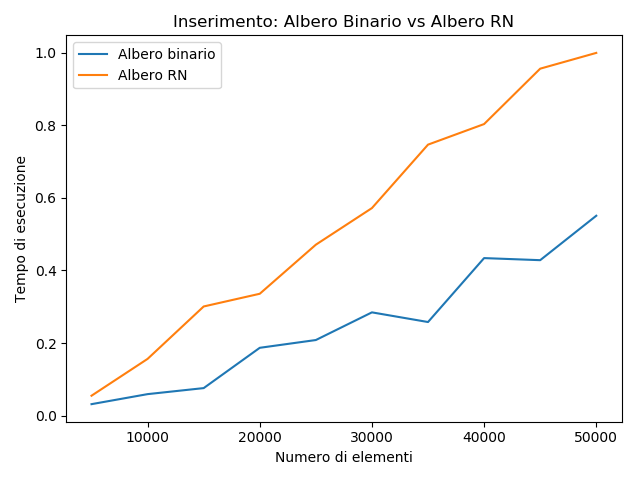
\includegraphics[scale=0.3]{Inserimentomedio}
		\caption{Caso medio per l'inserimento}
		\label{fig:InsMedio}
		\end{figure}
			
\subsection{Inserimento - Caso peggiore per ABR (Input in ord. decrescente)}
Grazie alla figura \ref{fig:InsPeggioreAbr} 
 		\begin{figure}[!htb]
		\centering
		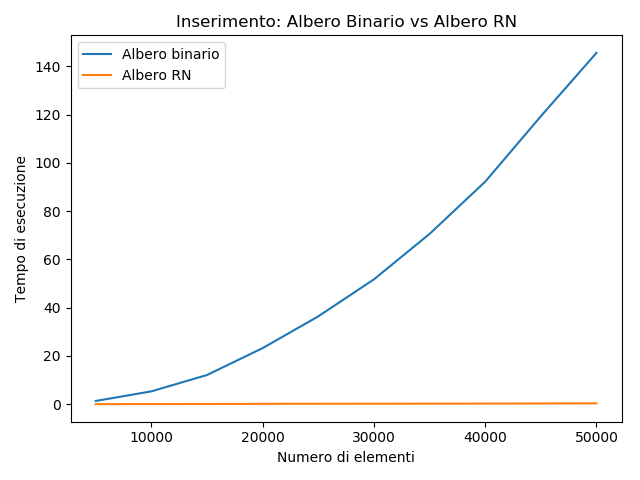
\includegraphics[scale=0.3]{Inserimentopeggiore}
		\caption{Caso peggiore per l'albero binario di ricerca}
		\label{fig:InsPeggioreAbr}
		\end{figure}
		
\subsection{Ricerca - Caso medio (input Random)}

		\begin{figure}[!htb]
		\centering
		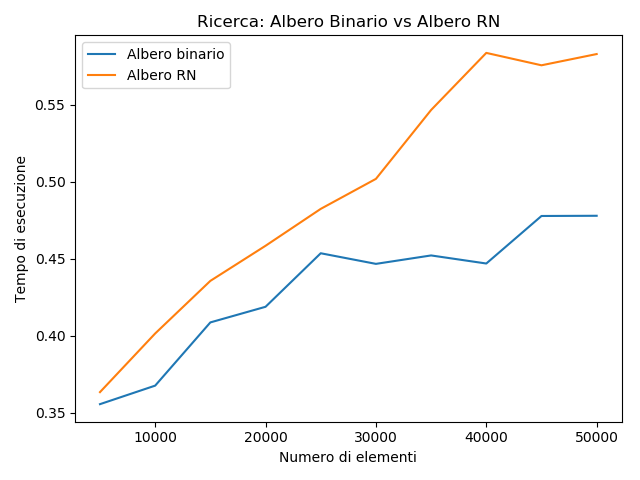
\includegraphics[scale=0.3]{Ricercamedio}
		\caption{Caso medio per la ricerca}
		\label{fig:RicercaMedio}
		\end{figure}
		

\subsection{Ricerca - Caso peggiore per ABR (ricerca su input in ord. decrescente)}		

		\begin{figure}[!htb]
		\centering
		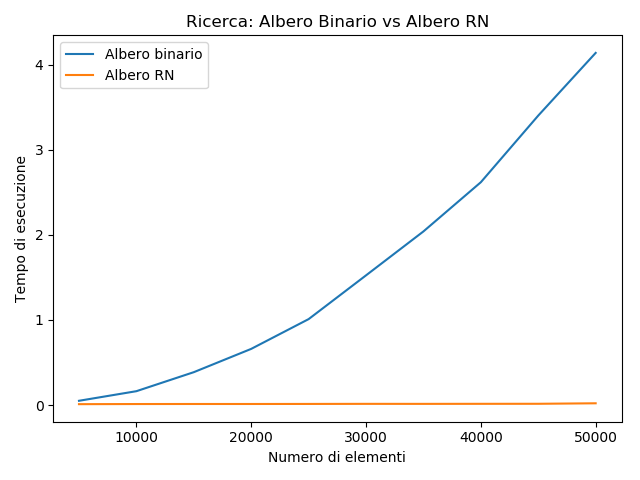
\includegraphics[scale=0.3]{casopeggioreABR}
		\caption{Caso peggiore per l'albero binario di ricerca}
		\label{fig:RicercaPeggioreAbr}
		\end{figure}
		

\section{Conclusioni}
E' stato verificato il comportamento asintotico degli algoritmi di inserimento e ricerca: si deduce che l'ARN e' preferibile quando si ipotizza un preordinamento (crescente o decrescente) nei valori in input: in tal caso l'ABR risulta totalmente sbilanciato e quindi sconveniente sia per inserimento che per ricerca. Se invece i valori in input non sono ordinati, avremo un ABR non eccessivamente sbilanciato: l'inserimento sara' spesso piu' veloce rispetto a quello del concorrente poiche', a differenza di esso, non deve eseguire un fix-up.
\end{document}
